\documentclass[11pt,aspectratio=169,xcolor=dvipsnames]{beamer}
\usepackage[utf8]{inputenc}
\usepackage{comment}
\usepackage{graphicx}
\usepackage{times}
\usepackage{amsmath}
\usepackage{import}
\usepackage{steinmetz}
\usepackage{booktabs}
\usepackage[official]{eurosym}
\usepackage[backend=biber,style=ieee,maxcitenames=3]{biblatex}
\usepackage{import}
\usepackage[caption=false,font=footnotesize,labelfont=sf,textfont=sf]{subfig}
\usepackage{caption}
\usepackage{tikz}
\usepackage[export]{adjustbox}
\usepackage{xcolor}
\usepackage{svg}
\usepackage{bookmark}
\usepackage[version=4]{mhchem}
\usepackage{ragged2e}
\usepackage{tabularx}
\usepackage{textcomp}
\usepackage{gensymb}
\usepackage{svg}

\renewcommand{\arraystretch}{1.5}
\bibliography{Electrolyzer}


\usefonttheme{professionalfonts}

\setbeamerfont{footnote}{size=\tiny}
\setbeamertemplate{footline}[frame number]
\setbeamertemplate{navigation symbols}{}
\usecolortheme[named=black]{structure}
\usefonttheme{structurebold}
\urlstyle{sf}

\setbeamertemplate{frametitle continuation}{}
\setbeamertemplate{section in toc}[sections numbered]
\makeatletter
\def\blfootnote{\xdef\@thefnmark{}\@footnotetext}
\makeatother

\renewcommand\multicitedelim{\addsemicolon\space}
\mode<presentation>
\usetheme{default}
\title[title]{Electrical Modeling of Alkaline and Proton Exchange Membrane Electrolyzers}
\author[Chowdhury]{Ushnish Chowdhury}
\subject{Designing an electrical model of an electrolyzer}
\date{October 4, 2024}

\AtBeginSection[]{\begin{frame}\tableofcontents[currentsection]\end{frame}} 
% --------------------------------------------------------------------
\begin{document}

% Title page
% --------------------------------------------------------------------
\begin{frame}
	\includegraphics[scale=.1]{Aalto_ELEC_EN_21_BLACK_1.png}\vspace{-.5Em}
	\titlepage
\end{frame}

%Contents
% --------------------------------------------------------------------
\begin{frame}{Contents}
	\begin{itemize}
        \item Overview of green hydrogen technology\vspace{0.5Em}
        \item Basic principle of electrolysis and electrolyzers\vspace{0.5Em}
        \item Electrical model of electrolyzers to represent static and dynamic behaviors \vspace{0.5Em}
        \item Showcasing simulation results (in PLECS)\vspace{0.5Em}
    \end{itemize}
\end{frame}
% ------------------------------------------------------------------------

\section{Green Hydrogen Technology}
%   \begin{frame} {Hydrogen Technology}
%     \begin{itemize}
%       \item Clean and efficient (up to 80\%) energy carrier \vspace{0.5Em}
%       \item Can be produced through thermochemical, electrolytic 
%       and biological processes \vspace{0.5Em}
%       \item Current applications \vspace{0.5Em}
%         \begin{itemize}
%           \item Fuel cells to generate electricity \vspace{0.3Em}
%           \item Decarbonizing industrial processes 
%           such as steel production, ammonia synthesis and
%           fertilizer manufacturing \vspace{0.3Em}
%           \item Powering long distance transportation 
%           like aviation, shipping \vspace{0.3Em}
%         \end{itemize}
%     \end{itemize} 
%   \end{frame} 

  % \begin{frame} {Hydrogen Spectra}
  %   \begin{figure}
  %   \centerline{\includegraphics[width=\textwidth, height=0.4\textwidth]{1200px-Grey_blue_green_hydrogen.jpg}}
  %   \end{figure}
  % \end{frame}

  \begin{frame}{Green Hydrogen Technology}
    \begin{center}
      \def\svgwidth{\textwidth}
      \input{green_hydrogen_technology.pdf_tex}
    \end{center}
  \end{frame}
  
  \begin{frame}{Hydrogen Production in Europe 
    \footfullcite{european_commission_directorate_general_for_energy_hydrogen_2020}}
    \begin{itemize}
    \item Current statistics \vspace{0.5Em}
        \begin{itemize}
        \item 11.5 Mt produced in 2022, with 96\% based on natural gas reforming \vspace{0.3Em}
        \item Only 0.3\% based on water electrolysis \vspace{0.3Em}
        \item Prime contributors: Germany, the Netherlands and Poland \vspace{0.5Em}
        \end{itemize}
    \item Targets for 2030 \vspace{0.5Em}
        \begin{itemize}
        \item Scale up production up to 10 Mt/year  \vspace{0.3Em}
        \item Directly connecting 80-120 GW of renewable energy production capacity to 
        electrolyzers \vspace{0.5Em}
        \end{itemize}
    \item Targets for 2050 \vspace{0.5Em}
        \begin{itemize}
        \item Increase renewable electrolyzer capacity to at least 500 GW
        \end{itemize}  
    \end{itemize}
  \end{frame}

\begin{frame}{Hydrogen Production in Finland 
  \footnote{Source: Hydrogen cluster Finland - h2cluster.fi}}
    \begin{itemize}
      \item Current statistics \vspace{0.5Em}
        \begin{itemize}
          \item 0.2 Mt/year, with 99\% based on natural gases \vspace{0.5Em}
        \end{itemize} 
      \item Targets for 2030 
      \vspace{0.5Em}
        \begin{itemize}
          \item Produce at least 10\% of EU's green hydrogen \vspace{0.3Em}
          \item 1 Mt production with a forecasted consumption of 12-98 TWh clean electricity \vspace{0.5Em}
        \end{itemize}
      \item Advantages for Finland \vspace{0.5Em}
        \begin{itemize}
          \item Abundance of renewable energy source, wind energy in particular \vspace{0.3Em}
          \item Availability of resource reserves \vspace{0.3Em}
          \item Expertise in designing cost-effective electrolyzers
        \end{itemize}  
    \end{itemize}
  \end{frame}

% \begin{frame}{Hydrogen production in Europe}
% \end{frame}  

\section{Basic Principle of Water Electrolysis}
  \begin{frame}{Basic Principle of Water Electrolysis}
    \begin{columns}[t]
      \begin{column}{.4\textwidth}
        \begin{itemize}
            \item Process of passing electric current through a substance 
            to induce a chemical change (oxidation and reduction) \vspace{0.5Em}
            \item Electrolyzer is a device which uses electrolysis to split water molecules 
            into hydrogen and oxygen \footnote{Water needs to be pre-processed; \\ 
            1 kg \ce{H_2} production requires $\approx$ 9 L processed water} \\ \vspace{1.5Em}
            \centerline{\ce{H_2O} (l) = \ce{H_2} (g) + \ce{1/2O_2} (g)}
        \end{itemize}
      \end{column}
      \begin{column}{.6\textwidth}
        \begin{center}
          \def\svgwidth{\textwidth}
          \input{general_electrolyzer.pdf_tex}
        \end{center}
      \end{column}
    \end{columns}     
  \end{frame}
  
  % \begin{frame}{Types of Electrolyzers}
  %   \begin{itemize}
  %     \item Distinguished based on type of electrolyte used
  %   \end{itemize}
  %   \begin{table}[h!]
  %       \begin{tabularx}{0.95\textwidth}{>{\raggedright\arraybackslash}X 
  %         |>{\centering\arraybackslash}X|>{\centering\arraybackslash}X|>{\centering\arraybackslash}X}
  %         \hline
  %         Comparison parameter & Alkaline Electrolyzer & PEM Electrolyzer & Solid Oxide Electrolyzer \\
  %         \hline
  %         Electrolyte & \ce{KOH}, \ce{NaOH} & Solid polymer & \ce{MgO-ZrO_2}\\
  %         \hline
  %         Temperature range (\degree \ C) & 70-90 & 50-80 & 650-850 \\
  %         \hline
  %         Current density ($\text{A/cm}^2$) & 0.2-0.5 & up to 20 & 0-2 \\
  %         \hline
  %         Efficiency (\%) & 60-80 & 80 & 100 * \\
  %         \hline
  %         Status & Established & Upcoming & R\&D\\
  %         \hline
  %       \end{tabularx}  
  %   \end{table}    
  % \end{frame}
  
  \begin{frame}{Alkaline and PEM Electrolyzers 
    \footnote{EU ban on perfluorosulfonic acid 
    can be a potential setback for PEM electrolyzer technology}}
    \begin{columns}
      \begin{column}{.5\textwidth}
        \begin{center}
          \def\svgwidth{0.8\textwidth}
          \input{general_aw_electrolyzer.pdf_tex}
        \end{center}
        % \begin{itemize}
        %   \item Consumption = 49 kWh/kg
        %   \item Current density = 0.7 $\text{A/cm}^2$
        %   \item Critical raw materials as catalyst = 0.3 mg/W
        % \end{itemize}
        \begin{itemize}
          \item Matured and widely commercialized
          \item Minimal capital expenditure
          \item Less flexible; low current density
        \end{itemize}    
      \end{column}
      \begin{column}{0.5\textwidth}
        \begin{center}
          \def\svgwidth{0.8\textwidth}
          \input{general_pem_electrolyzer.pdf_tex}
        \end{center}
        % \begin{itemize}
        %   \item Consumption = 52 kWh/kg
        %   \item Current density = 2.4 $\text{A/cm}^2$
        %   \item Critical raw materials as catalyst = 1.25 mg/W
        % \end{itemize}
          \begin{itemize}
            \item High current density; compact            
            \item Output hydrogen purity \textgreater 98 \%
            \item Expensive; use of rare metals
          \end{itemize}  
      \end{column}
    \end{columns}  
  \end{frame}

  % \begin{frame}{Need for Voltage Analysis}
  %   \begin{columns}[t]
  %     \begin{column}{.5\textwidth}
  %       \begin{itemize}
  %         \item Faraday's first law of electrolysis \\ \vspace{1.2Em}
  %         \centerline{$\dot{n}_{\ce{H_2}} = \eta\dfrac{jA}{n_{\text{e}}F} = 
  %         \eta\dfrac{i_{\text{E}}}{n_{\text{e}}F}$} \vspace{1.2Em}
  %         \item Efficiency, $\eta$ is presumed to be unity, not feasible for real-world systems \vspace{0.5Em}
  %         \item Reduced by stray currents and nonlinearities due to gas crossover through the diaphragm
  %       \end{itemize}
  %     \end{column}
  %     \begin{column}{.5\textwidth}
  %     \end{column}  
  %   \end{columns} 
  % \end{frame}

  % \begin{frame}{Electrolyzer Stack Voltage Equation}
  %   \centerline{$u_{\text{E}} = N_{\text{s}} (u_{\text{rev}} 
  %   + u_{\text{ohm}} + u_{\text{act}} + u_{\text{con}})$} \vspace{1.5Em}
  %   \begin{itemize}
  %     \item Reversible voltage, $u_{\text{rev}}$ is the minimum electrolysis initiation voltage \vspace{0.3Em}
  %     \item Ohmic overvoltage, $u_{\text{ohm}}$ refers to the ohmic losses \vspace{0.3Em}
  %     \item Activation overvoltage, $u_{\text{act}}$ is produced due to kinetic losses in the electrodes \vspace{0.3Em}
  %     \item Concentration overvoltage, $u_{\text{con}}$ restricts the generation of current due to mass 
  %     transport effect, negligible incase of electrolyzers due to low current densities \vspace{0.3Em}
  %   \end{itemize}  
  % \end{frame}

\section{Electrical Modeling of Electrolyzers}
  
  % \begin{frame}{Common Static Electrical Model \footnote{Applicable for both AEL and PEMEL}}
  %   \begin{columns}
  %     \begin{column}{0.6\textwidth}
  %       \begin{center}
  %         \def\svgwidth{0.6\textwidth}
  %         \input{simple_electrical_model_electrolyzer.pdf_tex}
  %       \end{center}
  %     \end{column}
  %     \begin{column}{0.4\textwidth}
  %       \begin{center}
  %         \begin{align*}
  %           u_{\text{E}} &= i_{\text{E}} Z(s) + u_{\text{rev}} \\
  %           => u_{\text{E}} &= i_{\text{E}} R + u_{\text{rev}}
  %         \end{align*}
  %       \end{center}    
  %     \end{column}
  %   \end{columns} \vspace{1Em}
  %   \begin{itemize}
  %     \item Assumes operation under constant temperature and pressure \vspace{0.3Em}
  %     \item Impedance considered purely resistive, $Z(s) = R$ \vspace{0.3Em}
  %     \item Nonlinearities and dynamic behaviors not considered \vspace{0.3Em}
  %   \end{itemize} 
  % \end{frame}
  
  \begin{frame}{Dynamic Model for Alkaline and PEM Electrolyzers}
    \begin{center}
      \def\svgwidth{0.53\textwidth}
      \input{static-dynamic-model-electrolyzer.pdf_tex}
    \end{center}
    \begin{align*}
      u_{\text{E}} = u_{\text{rev}} + u_{\text{ohm}} + u_{\text{act}} 
    \end{align*}
    \begin{itemize}
      \item Helps acquiring relevant data regarding energy consumption under various operating conditions \vspace{0.3Em}
      %\item Can be used for the design and development of efficient power supplies \vspace{0.3Em}
    \end{itemize} 
  \end{frame}
  
  % \begin{frame}{Reversible Voltage ($ u_{\text{rev}}$)}
  %   \begin{itemize}
  %     \item Also referred as the open circuit voltage (OCV) \vspace{0.3Em}
  %     \item Thermodynamic expression \\ \vspace{1.2Em}
  %     \begin{center} 
  %       $u_{\text{rev}} = \dfrac{\Delta G}{n_{\text{e}}F}$ \\ \vspace{1.2Em}
  %     \end{center}  
  %     where $\Delta G = \Delta H - Q = \Delta H - T \Delta S$ \vspace{0.3Em}
  %     \item The parameter $\Delta G$ is dependent on $T$ and reacting chemical species 
  %     activity $a$, forming the equation \\ \vspace{1.2Em}
  %     \begin{center}
  %       $ u_{rev} = u_{rev}^0 + \dfrac{\Re T}{n_{\text{e}}F}\ln{\dfrac{a_{\text{ox}}}{a_{\text{re}}}}$
  %     \end{center}  
  %   \end{itemize}  
  % \end{frame}
  
  % \begin{frame}{Implementation on Electrolyzer Electrodes}
  %   \begin{table}[h!]
  %     \begin{tabularx}{\textwidth}{>{\raggedright\arraybackslash}X 
  %       |>{\centering\arraybackslash}X|>{\centering\arraybackslash}X}
  %       \hline
  %       Equation & AWE & PEMWE \\
  %       \hline
  %       Anodic ($u_{rev,a}$) & 
  %       ${u^0_{\text{rev,a}}} + f(T)\ln{\dfrac{a^{1/2}_{\ce{O_2}}a_{\ce{H_2O}}} {a^2_{\ce{OH}^{-}}}}$ & 
  %       ${u^0_{\text{rev,a}}} + f(T)\ln{\dfrac{a^{1/2}_{\ce{O_2}}a^2_{\ce{H^+}}} {a_{\ce{H_2O}}}}$ \\ [2ex]
  %       \hline
  %       Cathodic ($u_{rev,c}$) & 
  %       ${u^0_{\text{rev,c}}} + f(T)\ln{\dfrac{a^2_{\ce{H_2O}}}{a_{\ce{H_2}} a_{\ce{OH}^{-}}^2}}$ &
  %       ${u^0_{\text{rev,c}}} + f(T)\ln{\dfrac{a^2_{\ce{H^+}}}{a_{\ce{H_2}}}}$ \\ [2ex]
  %       \hline
  %       Total ($u_{\text{rev,a}} - u_{\text{rev,c}}$) & 
  %       ${u^0_{\text{rev}}} + f(T)\ln{\dfrac{a^2_{\ce{H_2}}a^{1/2}_{\ce{O_2}}}{a_{\ce{H_2O}}}} $ &
  %       ${u^0_{\text{rev}}} + f(T)\ln{\dfrac{a^2_{\ce{H_2}}a^{1/2}_{\ce{O_2}}}{a_{\ce{H_2O}}}} $ \\ [2ex]
  %       \hline
  %     \end{tabularx}  
  %   \end{table}
  %   \begin{flushright}
  %     where $f(T) = \dfrac{\Re T}{n_{\text{e}}F}$
  %   \end{flushright}  
  % \end{frame}

  % \begin{frame}{Standard Reversible Voltage ($u^0_{\text{rev}}$)}
  %   \begin{columns}
  %     \begin{column}{0.4\textwidth}
  %       \begin{itemize}
  %         \item Reference reversible voltage as a function of temperature at standard pressure of 1 bar 
  %         \vspace{0.3Em}
  %         \item Derived experimentally or through approximations  \vspace{0.3Em}
  %         \item All of the equations exhibit minimal differences in output when operated within
  %         the designated temperature range \vspace{0.3Em}
  %       \end{itemize}  
  %     \end{column}
  %     \begin{column}{0.6\textwidth}
  %       \begin{center}
  %         \def\svgwidth{0.6\columnwidth}
  %         \tiny \input{standard_rev_voltage.pdf_tex}
  %       \end{center}
  %     \end{column}  
  %   \end{columns}  
  % \end{frame}
  
  % \begin{frame}{Relation to Pressure}
  %   \begin{columns}
  %     \begin{column} {0.5\textwidth}
  %       \begin{itemize}
  %         \item Activity of an ideal gas
  %         \begin{center}
  %           $a_\text{X} = \dfrac{p_{X}}{p^0}$ \vspace{0.7Em}
  %         \end{center}
  %         where $p^0 = 1 \ \text{bar}$  \vspace{1.5Em}
  %         \item Activity of pure liquid water
  %         \begin{center}
  %           $a_{\ce{H_2O}\text{,E}} = \dfrac{p_{\text{sv,E}}(T, m)}{p_{\text{sv}}(T)}$ \vspace{0.7Em}
  %         \end{center}
  %         For PEMWE $a_{\ce{H_2O}\text{,E}} = 1$
  %       \end{itemize}  
  %     \end{column}
  %     \begin{column} {0.5\textwidth}
  %       Partial pressures of hydrogen and oxygen \\ \vspace{0.5Em}
  %       \begin{itemize}
  %         \item For PEMWE
  %         \begin{center}
  %           $p_{\ce{H_2}} = p_{\text{c}} - p_{\text{sv}}(T)$ \\ \vspace{0.3Em}
  %           $p_{\ce{O_2}} = p_{\text{a}} - p_{\text{sv}}(T)$ \vspace{1.2Em}
  %         \end{center}  
  %         \item For AWE
  %         \begin{center}
  %           $p_{\ce{H_2}} = p_{\ce{O_2}} = p - p_{\text{sv, E}}(T, m)$
  %         \end{center}  
  %       \end{itemize}  
  %     \end{column}  
  %   \end{columns}     
  % \end{frame}
  
  % \begin{frame} {Calculating Saturated Vapour Pressure ($p_{\text{sv}}$)}
  %   \begin{itemize}
  %     \item For temperature range of $1-100 \ \degree \text{C}$ \vspace{1Em}
  %     \begin{center}
  %       $\log_{10} p_{\text{sv}}(T) = 35.4462 - \dfrac{3343.93 \, \text{K}}{T}
  %       - 10.9 \log_{10}T + (4.1645\cdot10^{-3} \, \text{K}^{-1})T $ \vspace{1Em}
  %     \end{center}
  %     \item Vapour pressure of the electrolyte in AWE \vspace{1Em}
  %     \begin{center}
  %       $p_{\text{sv,E}}(T,m) = 10^{\text{a}}p_{\text{sv}}(T)^{\text{b}}$ \vspace{1Em}
  %     \end{center}
  %     \, where $\text{a}$ and $\text{b}$ depends on electrolyte type and molality $m$  
  %   \end{itemize}  
  % \end{frame}
  
  % \begin{frame} {Reversible Voltage} 
  %   \begin{columns}
  %     \begin{column} {0.75\textwidth}
  %       \begin{itemize}
  %         \item For Alkaline electrolyzer stack \\ \vspace{1Em}
  %         $ N_{\text{s}} \left[u^0_{\text{rev}} + 
  %         f(T)\ln{\dfrac{(p - p_{\text{sv,E}}(T,m))^{3/2}p_{\text{sv}}(T)}{(p^{0})^{3/2}p_{\text{sv,E}}(T,m)}} \right]$ \vspace{1Em}
  %         \item For PEM electrolyzer stack \\ \vspace{1Em}
  %         $ N_s \left[u^0_{\text{rev}} + f(T)\ln{\dfrac{(p_{\text{c}} - p_{\text{sv}}(T))
  %         (p_{\text{a}} - p_{\text{sv}}(T))^{1/2}}{(p^{0})^{3/2}}} \right]$ \vspace{1Em}
  %         \item $u_{\text{rev}} = 1.229 \ \text{V}$ at standard operating conditions
  %       \end{itemize}  
  %     \end{column}
  %     \begin{column} {0.25\textwidth}
  %       \begin{flushright}
  %         \def\svgwidth{1.2\linewidth}
  %         \input{reversible_voltage_equivalent_circuit.pdf_tex}
  %       \end{flushright} 
  %     \end{column}  
  %   \end{columns}  
  % \end{frame}
  \begin{frame} {Reversible Voltage}
    \begin{itemize}
      \item Minimum electrolysis initiation voltage, derived from thermodynamics 
      of electrochemical reactions  \vspace{0.3Em}
      \item Calculated by combining anodic and cathodic half reactions potentials \vspace{0.3Em}
      \item 1.229 V at standard operating conditions (25\degree C, 1 bar) 
      \footfullcite{JARVINEN202231985} \vspace{0.3Em}
    \end{itemize} \vspace{1Em}
    \begin{columns}
      \begin{column}{0.5\textwidth} 
        \begin{center}
          \def\svgwidth{0.7\textwidth}
          \input{reversible_voltage_equivalent_circuit.pdf_tex}
        \end{center}  
      \end{column}
      \begin{column}{0.5\textwidth}
        \begin{align*}
          u_{\text{rev}} &= u^0_{\text{rev}} 
          +\dfrac{\bar{R} T}{n_{\text{e}}F}\ln{\dfrac{p}{p^0}} \\[7pt]
          &\text{where \,} u^0_{\text{rev}} \text{\, is the} \\
          &\text{standard reversible voltage}
        \end{align*}
      \end{column}
    \end{columns}
  \end{frame}  

  % \begin{frame}{Ohmic Overvoltage}
  %   \begin{columns}
  %     \begin{column}{0.6\textwidth}
  %       \begin{itemize}
  %         \item Resistance to electron and ion flow in the systems \vspace{0.5Em}
  %         \item Increases linearly following Ohm's law \vspace{1Em}
  %         \begin{center}
  %           $u_{\text{ohm,E}} = i_{\text{E}} R_{\text{ohm,E}}$
  %         \end{center}  \vspace{1Em}
  %         where $R_{\text{ohm,E}} = N_{\text{s}} R_{\text{ohm}} = N_{\text{s}} \dfrac{r}{A}$ \vspace{0.5Em}
  %         \item Area specific resistance is expressed as a function of temperature \vspace{1Em}
  %         \begin{center}
  %           $r = r_1 + r_2T + \dfrac{r_3}{T} + \dfrac{r_4}{T^2}$ \vspace{1Em}
  %         \end{center}   
  %       \end{itemize}
  %     \end{column}
  %     \begin{column}{0.4\textwidth}
  %       \begin{center}
  %         \def\svgwidth{\linewidth}
  %         \input{ohmic_effects.pdf_tex}
  %       \end{center} 
  %     \end{column}  
  %   \end{columns}    
  % \end{frame}

  \begin{frame}{Ohmic Overvoltage}
    \begin{itemize}
      \item Resistance to electron and ion flow in the system \vspace{0.3Em}
      \item Increases linearly following Ohm's law \vspace{0.3Em}
      \item Area specific resistance is expressed as a function of temperature \vspace{1Em}
        \begin{center}
            $r = r_1 + r_2T + \dfrac{r_3}{T} + \dfrac{r_4}{T^2}$ \vspace{1Em}
        \end{center}
        % \begin{flushright}
        %     where $r_1, r_2, r_3$ and $r_4$ are adjusted based on experimental data 
        %     %\footfullcite{iribarren_dynamic_modeling_2023}
        % \end{flushright}
    \end{itemize} \vspace{1Em}
    \begin{columns}
      \begin{column}{0.5\textwidth}
        \begin{center}
          \def\svgwidth{0.7\textwidth}
          \input{ohmic_effects.pdf_tex}
        \end{center}
      \end{column}
      \begin{column}{0.5\textwidth}
        \begin{align*}
          u_{\text{ohm}} & = i_{\text{E}} R_{\text{ohm}} = i_{\text{E}} \dfrac{r}{A} \\
          & \text{where \,} A \text{\, is the electrolyzer cell area}
        \end{align*}
      \end{column}
    \end{columns}  
  \end{frame}  
  
  % \begin{frame} {Activation Overvoltage ($u_{\text{act}}$)}
  %   \begin{itemize}
  %     \item Additional energy required to overcome energy barriers associated 
  %     with chemical reaction at electrodes \vspace{1.5Em}
  %     \begin{center}
  %       $i_{\text{E}} = i^0_{\text{\text{i}}} \left[\exp\left(\dfrac{\alpha n_{\text{e}}F}{\Re T} u_{\text{\text{act,\text{i}}}}\right) 
  %       - \exp\left(\dfrac{(1-\alpha) n_{\text{e}}F}{\Re T}u_{\text{\text{act,\text{i}}}}\right)\right]$ \vspace{1.5Em}
  %     \end{center}
  %     \item Simplified through approximations \vspace{1Em}
  %       \begin{columns}
  %         \begin{column}{0.5\textwidth}
  %           \qquad \qquad In terms of voltage \\ \vspace{1.5Em}
  %           \begin{center} 
  %             $u_{\text{act,\text{i}}} = \dfrac{\Re T}{\alpha n_{\text{e}}F} \ln{\dfrac{i_{\text{E}}}{i^0_{\text{i}}}}$ \\ \vspace{1.5Em}
  %           \end{center}  
  %         \end{column}
  %         \begin{column}{0.5\textwidth}
  %           \qquad In terms of current \\ \vspace{1.5Em}
  %           \begin{center} 
  %             $ i_{\text{act,\text{i}}} = t_{\text{i}}\left[\exp\left( \frac{u_{\text{act,\text{i}}}}
  %           {s_{\text{i}}}\right) - 1 \right]$ \\ \vspace{1.5Em}
  %           \end{center}
  %           where $s_{\text{i}}$ and $t_{\text{i}}$ are parameters derived experimentally
  %         \end{column}  
  %       \end{columns}       
  %   \end{itemize}
  % \end{frame}

  % \begin{frame}{Electrical Double Layer Effect}
  %   \begin{center}
  %     \def\svgwidth{0.32\linewidth}
  %     \input{edl_equivalent_circuit.pdf_tex}
  %   \end{center}  
  %   \begin{itemize}
  %     \item Formed at the electrode-electrolyte interface \vspace{0.3Em}
  %     \item Introduces dielectric behavior in the system \vspace{0.3Em}
  %     \item Capacitor is placed in parallel to $u_{\text{act}}$ \vspace{1.5Em}
  %     \begin{center}
  %       $\dfrac{du_{\text{act,\text{i}}}(t)}{dt} = - \dfrac{1}{C_{\text{dl,i}}}
  %       \left(i_{\text{act,\text{i}}}\left(u_{\text{act,\text{i}}}(t)\right) - i_{E}(t)\right)$
  %     \end{center}  
  %   \end{itemize}
  % \end{frame}
  
  % \begin{frame}{Overall Equivalent Circuit for $u_{\text{act}}$}
  %   \begin{center}
  %     \def\svgwidth{0.7\linewidth}
  %     \input{activation_overvoltage_equivalent_circuit.pdf_tex} \vspace{1Em}
  %   \end{center}
  %   \begin{center}
  %     $u_{act, E} = N_s \left[s_{a}\ln\left( \dfrac{1}{t_a}i_{act,a}+1\right) 
  %     + s_{c}\ln\left( \dfrac{1}{t_c}i_{act,c}+1\right)\right]$
  %   \end{center}      
  % \end{frame}
\begin{frame}{Activation Overvoltage}
  \begin{itemize}
    \item Formed at the electrode-electrolyte interface, voltage required to overcome 
    reaction energy barriers \footfullcite{URSUA201218598} \vspace{0.3Em}
    \item Causes double-layer effect, modeled by the capacitors $C_{\text{dl,a}}$ 
    and $C_{\text{dl,c}}$ \vspace{0.3Em}
  \end{itemize}
  \begin{columns}
    \begin{column}{0.5\textwidth}
      \begin{align*}
        u_{\text{act,\text{x}}} &= s_{\text{x}} 
        \ln\left(\dfrac{1}{t_{\text{x}}} i_{\text{E}} + 1\right) \\[7pt]
        \text{or \,} i_{\text{act,\text{x}}} & = t_{\text{x}}\left[\exp\left( \frac{u_{\text{act,\text{x}}}}
        {s_{\text{x}}}\right) - 1 \right] \\[7pt] 
        C_{\text{dl,x}} &\frac{du_{\text{act,\text{x}}}(t)}{dt} = i_{\text{E}} - i_{\text{act,x}}
      \end{align*}
    \end{column}
    \begin{column}{0.5\textwidth}
      \begin{center}
        \def\svgwidth{\textwidth}
        \input{activation_overvoltage_equivalent_circuit.pdf_tex}
      \end{center}
    \end{column}
  \end{columns}
\end{frame}

\begin{frame}{State-space Representation}
  \begin{align*}
          C_{\text{dl,a}} \frac{du_{\text{act,a}}}{dt} &= i_{\text{E}} - i_{\text{act,a}}(u_{\text{act,a}}) \\[5pt]
          C_{\text{dl,c}} \frac{du_{\text{act,c}}}{dt} &= i_{\text{E}} - i_{\text{act,c}}(u_{\text{act,c}}) \\[5pt]
          u_{\text{E}} &= R_{\text{ohm}}i_{\text{E}} + u_{\text{act,a}} + u_{\text{act,c}} + u_{\text{rev}} \\[10pt]
          \text{where the current \,} & i_{E} \text{\, is the input and the voltage \,} u_E \text{\, is the output}    
  \end{align*}    
\end{frame}

% \begin{frame}{Limitations}
%     % \item Advantages \vspace{0.3Em}
%     %   \begin{itemize}
%     %     \item Helps acquiring relevant data regarding energy consumption under various operating conditions \vspace{0.3Em}
%     %     \item Can be used for the design and development of efficient power supplies \vspace{0.3Em}
%     %   \end{itemize} \vspace{0.5Em}
%       \begin{itemize}
%         \item Parameterization by Electrochemical impedance spectroscopy \vspace{0.3Em}
%         \item Deviation from experimental data at higher current densities; concentration 
%         losses not taken into account \vspace{0.3Em}
%         \item Further development required to increase accuracy for high power stack behavior \vspace{0.3Em}
%         \item Increase in model complexity for better representation of dynamic behavior \vspace{0.3Em}
%       \end{itemize}
% \end{frame}

% \begin{frame} {Parameterization}
%   \begin{itemize}
%     \item Electrochemical impedance spectroscopy (EIS) used to assume linearized impedance
%     % \begin{align*}
%     %     Z(\omega) = &R_{\text{E}} + \dfrac{R_{\text{act,a,E}}}{1 + (\omega R_{\text{act,a,E}}C_{\text{dl,a,E}})^2} 
%     %     + \dfrac{R_{\text{act,c,E}}}{1 + (\omega R_{\text{act,c,E}}C_{\text{dl,c,E}})^2} \\
%     %     & -j\left(\dfrac{\omega R_{\text{act,a,E}}^2 C_{\text{dl,a,E}}}{1 + (\omega R_{\text{act,a,E}}C_{\text{dl,a,E}})^2}
%     %     + \dfrac{\omega R_{\text{act,c,E}}^2 C_{\text{dl,c,E}}}{1 + (\omega R_{\text{act,c,E}}C_{\text{dl,c,E}})^2} \right) \\[10pt]
%     %     \text{where \,} & C_{\text{dl,a,E}} = \dfrac{C_{\text{dl,a}}}{N_{\text{s}}} \text{\, and \,} 
%     %     C_{\text{dl,c,E}} = \dfrac{C_{\text{dl,c}}}{N_{\text{s}}} \\[5pt]
%     %     & R_{\text{act,a,E}} = N_{\text{s}} R_{\text{act,a}} \text{\, and \,} 
%     %     R_{\text{act,c,E}} = N_{\text{s}} R_{\text{act,c}}
%     % \end{align*}
%     \begin{align*}
%       Z(s) &= \dfrac{u(s)}{i(s)} =  R_{\text{ohm}} + \dfrac{R_{\text{a}}}{sR_{\text{a}}+1} + \dfrac{R_{\text{c}}}{sR_{\text{c}}+1} 
%     \end{align*}  
%     \item Identification of parameters ($r, s, t$) done by adjusting the impedance values
%   \end{itemize}  
% \end{frame}

\section{Simulation Results}
  \begin{frame}{Model in PLECS}
    \begin{center}
      \includegraphics[scale=.35]{model-in-plecs.png} 
    \end{center}
  \end{frame}
  
  \begin{frame}{Simulation Results}
    \begin{columns}
      \begin{column}{0.5\textwidth}
        \begin{center}
          \small{Constant pressure = 25 bar \\ Temperatures = 15 \degree C, 65 \degree C} 
          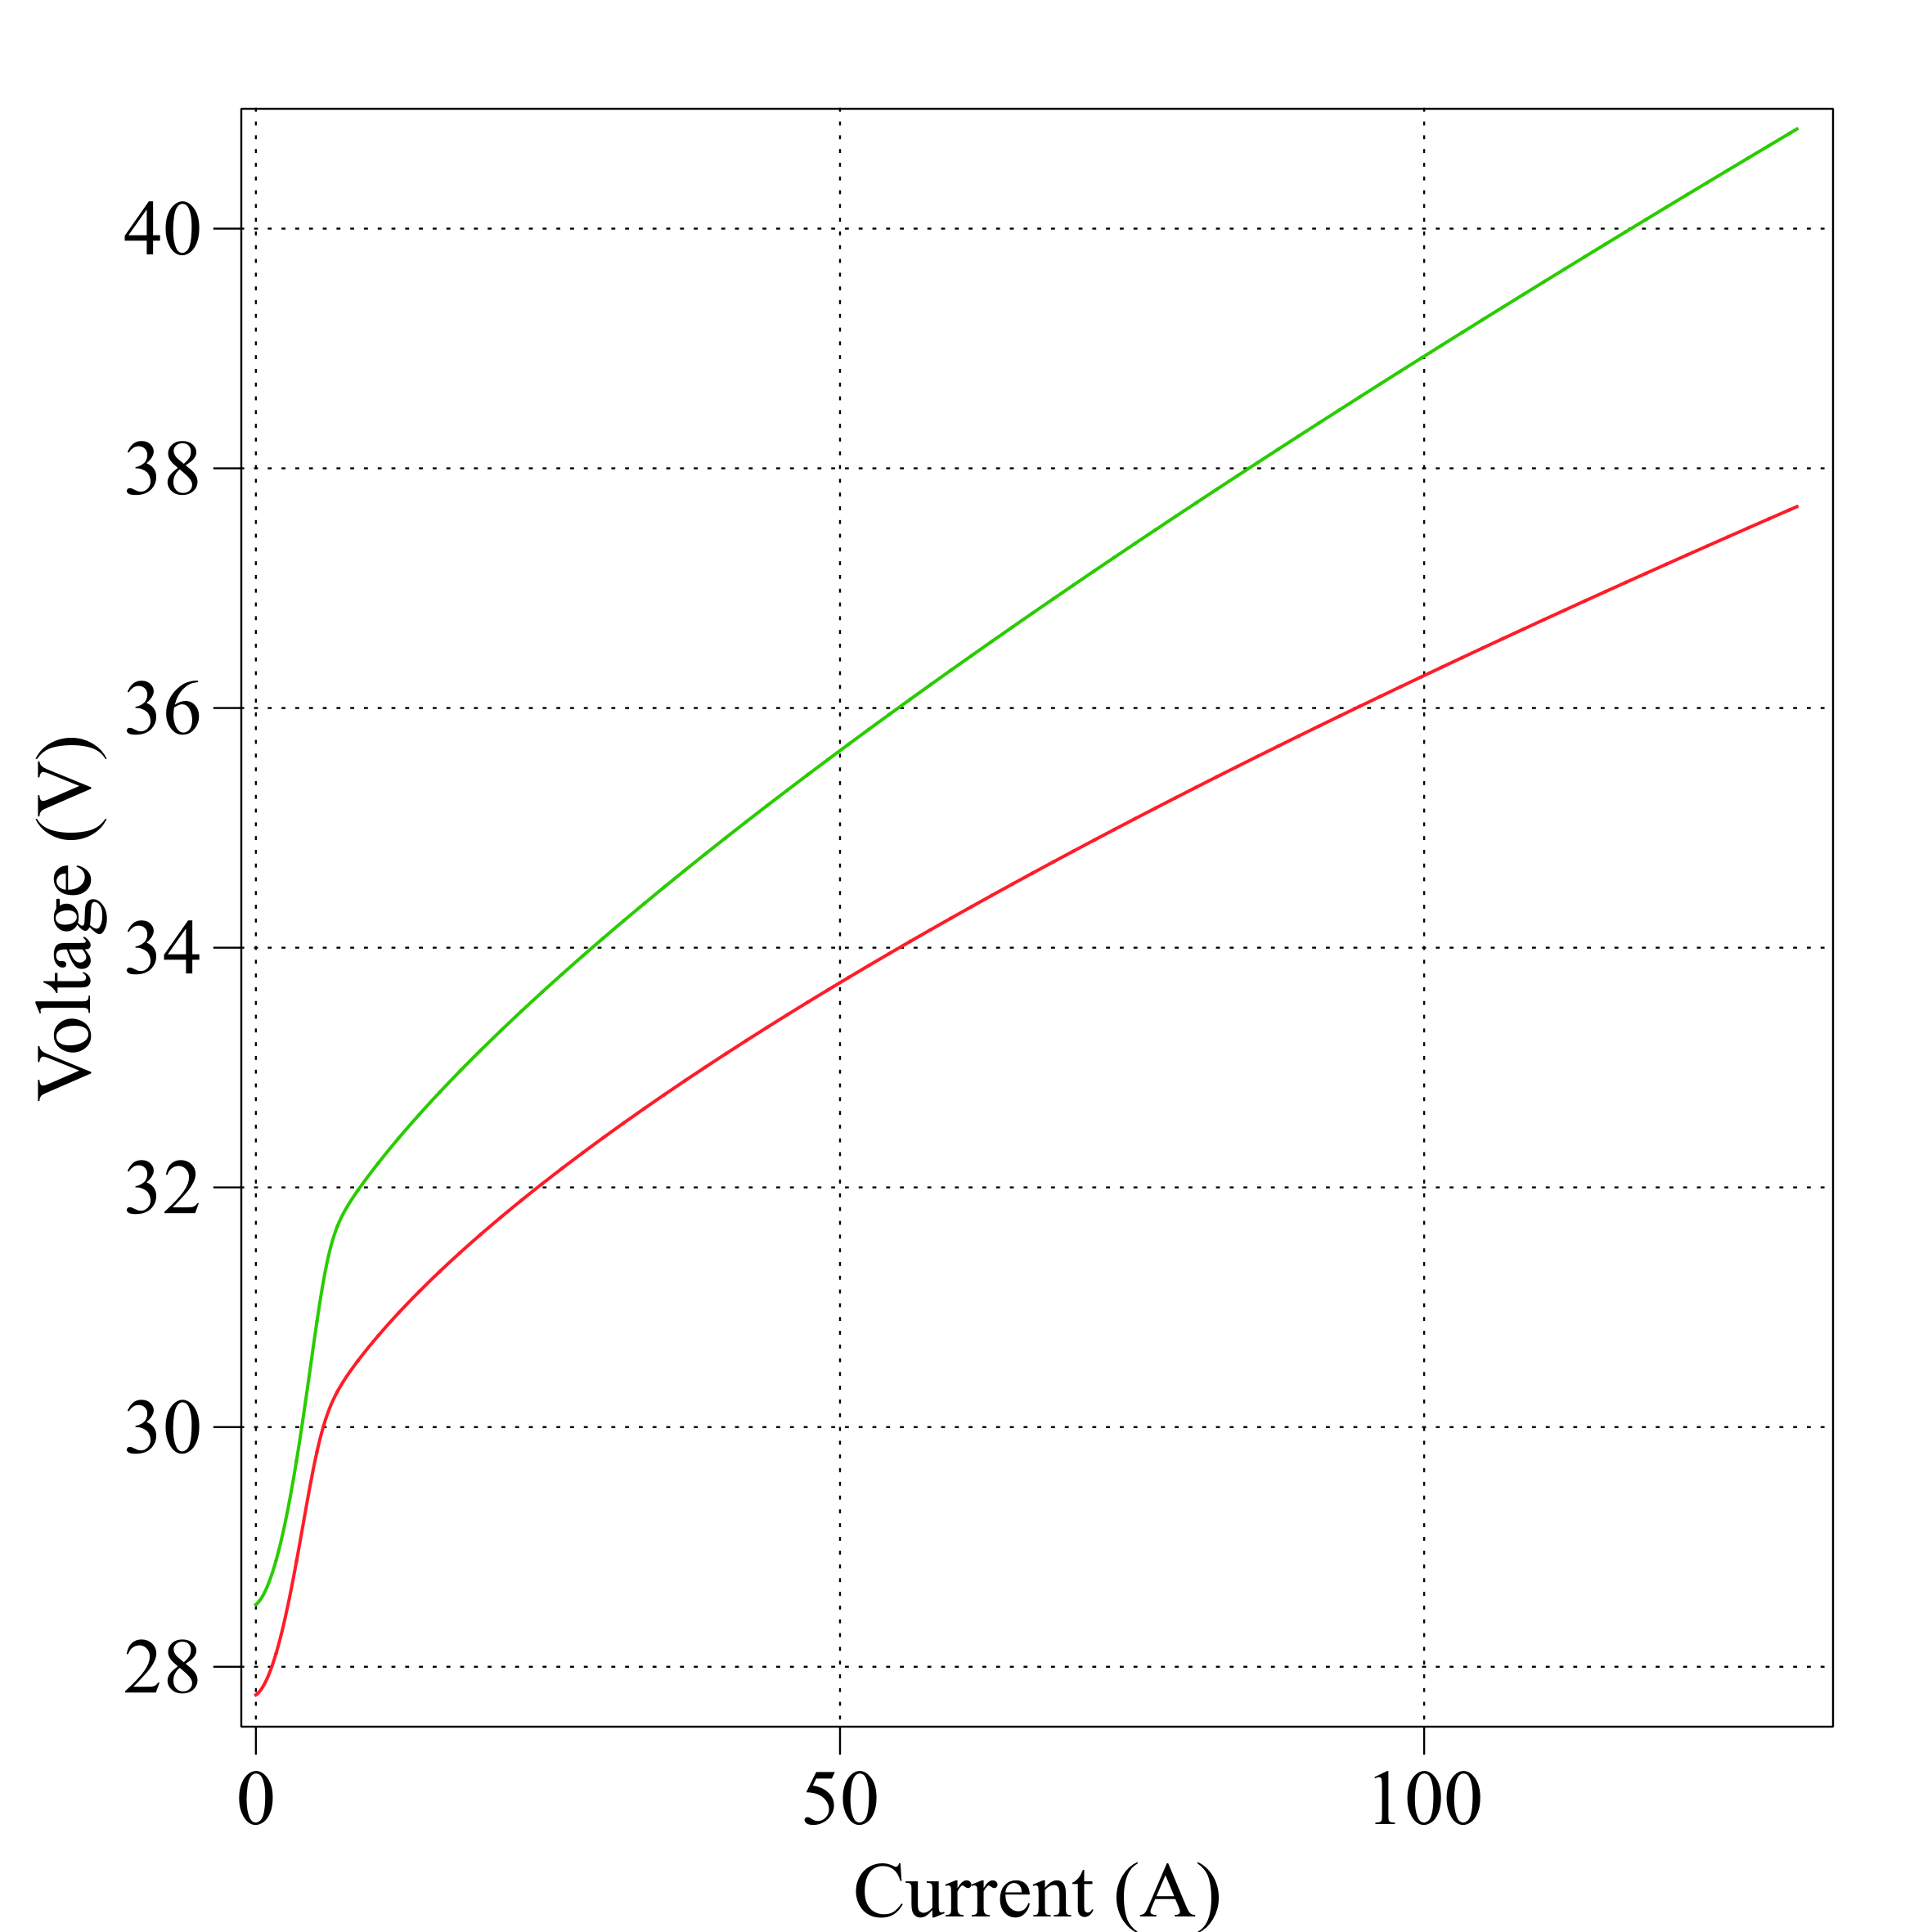
\includegraphics[scale=0.65]{scope-constant-pressure.png} 
        \end{center}
      \end{column}
      \begin{column}{0.5\textwidth}
        \begin{center}
          \small{Constant temperature = 65 \degree C \\ Temperatures = 5 bar, 25 bar} 
          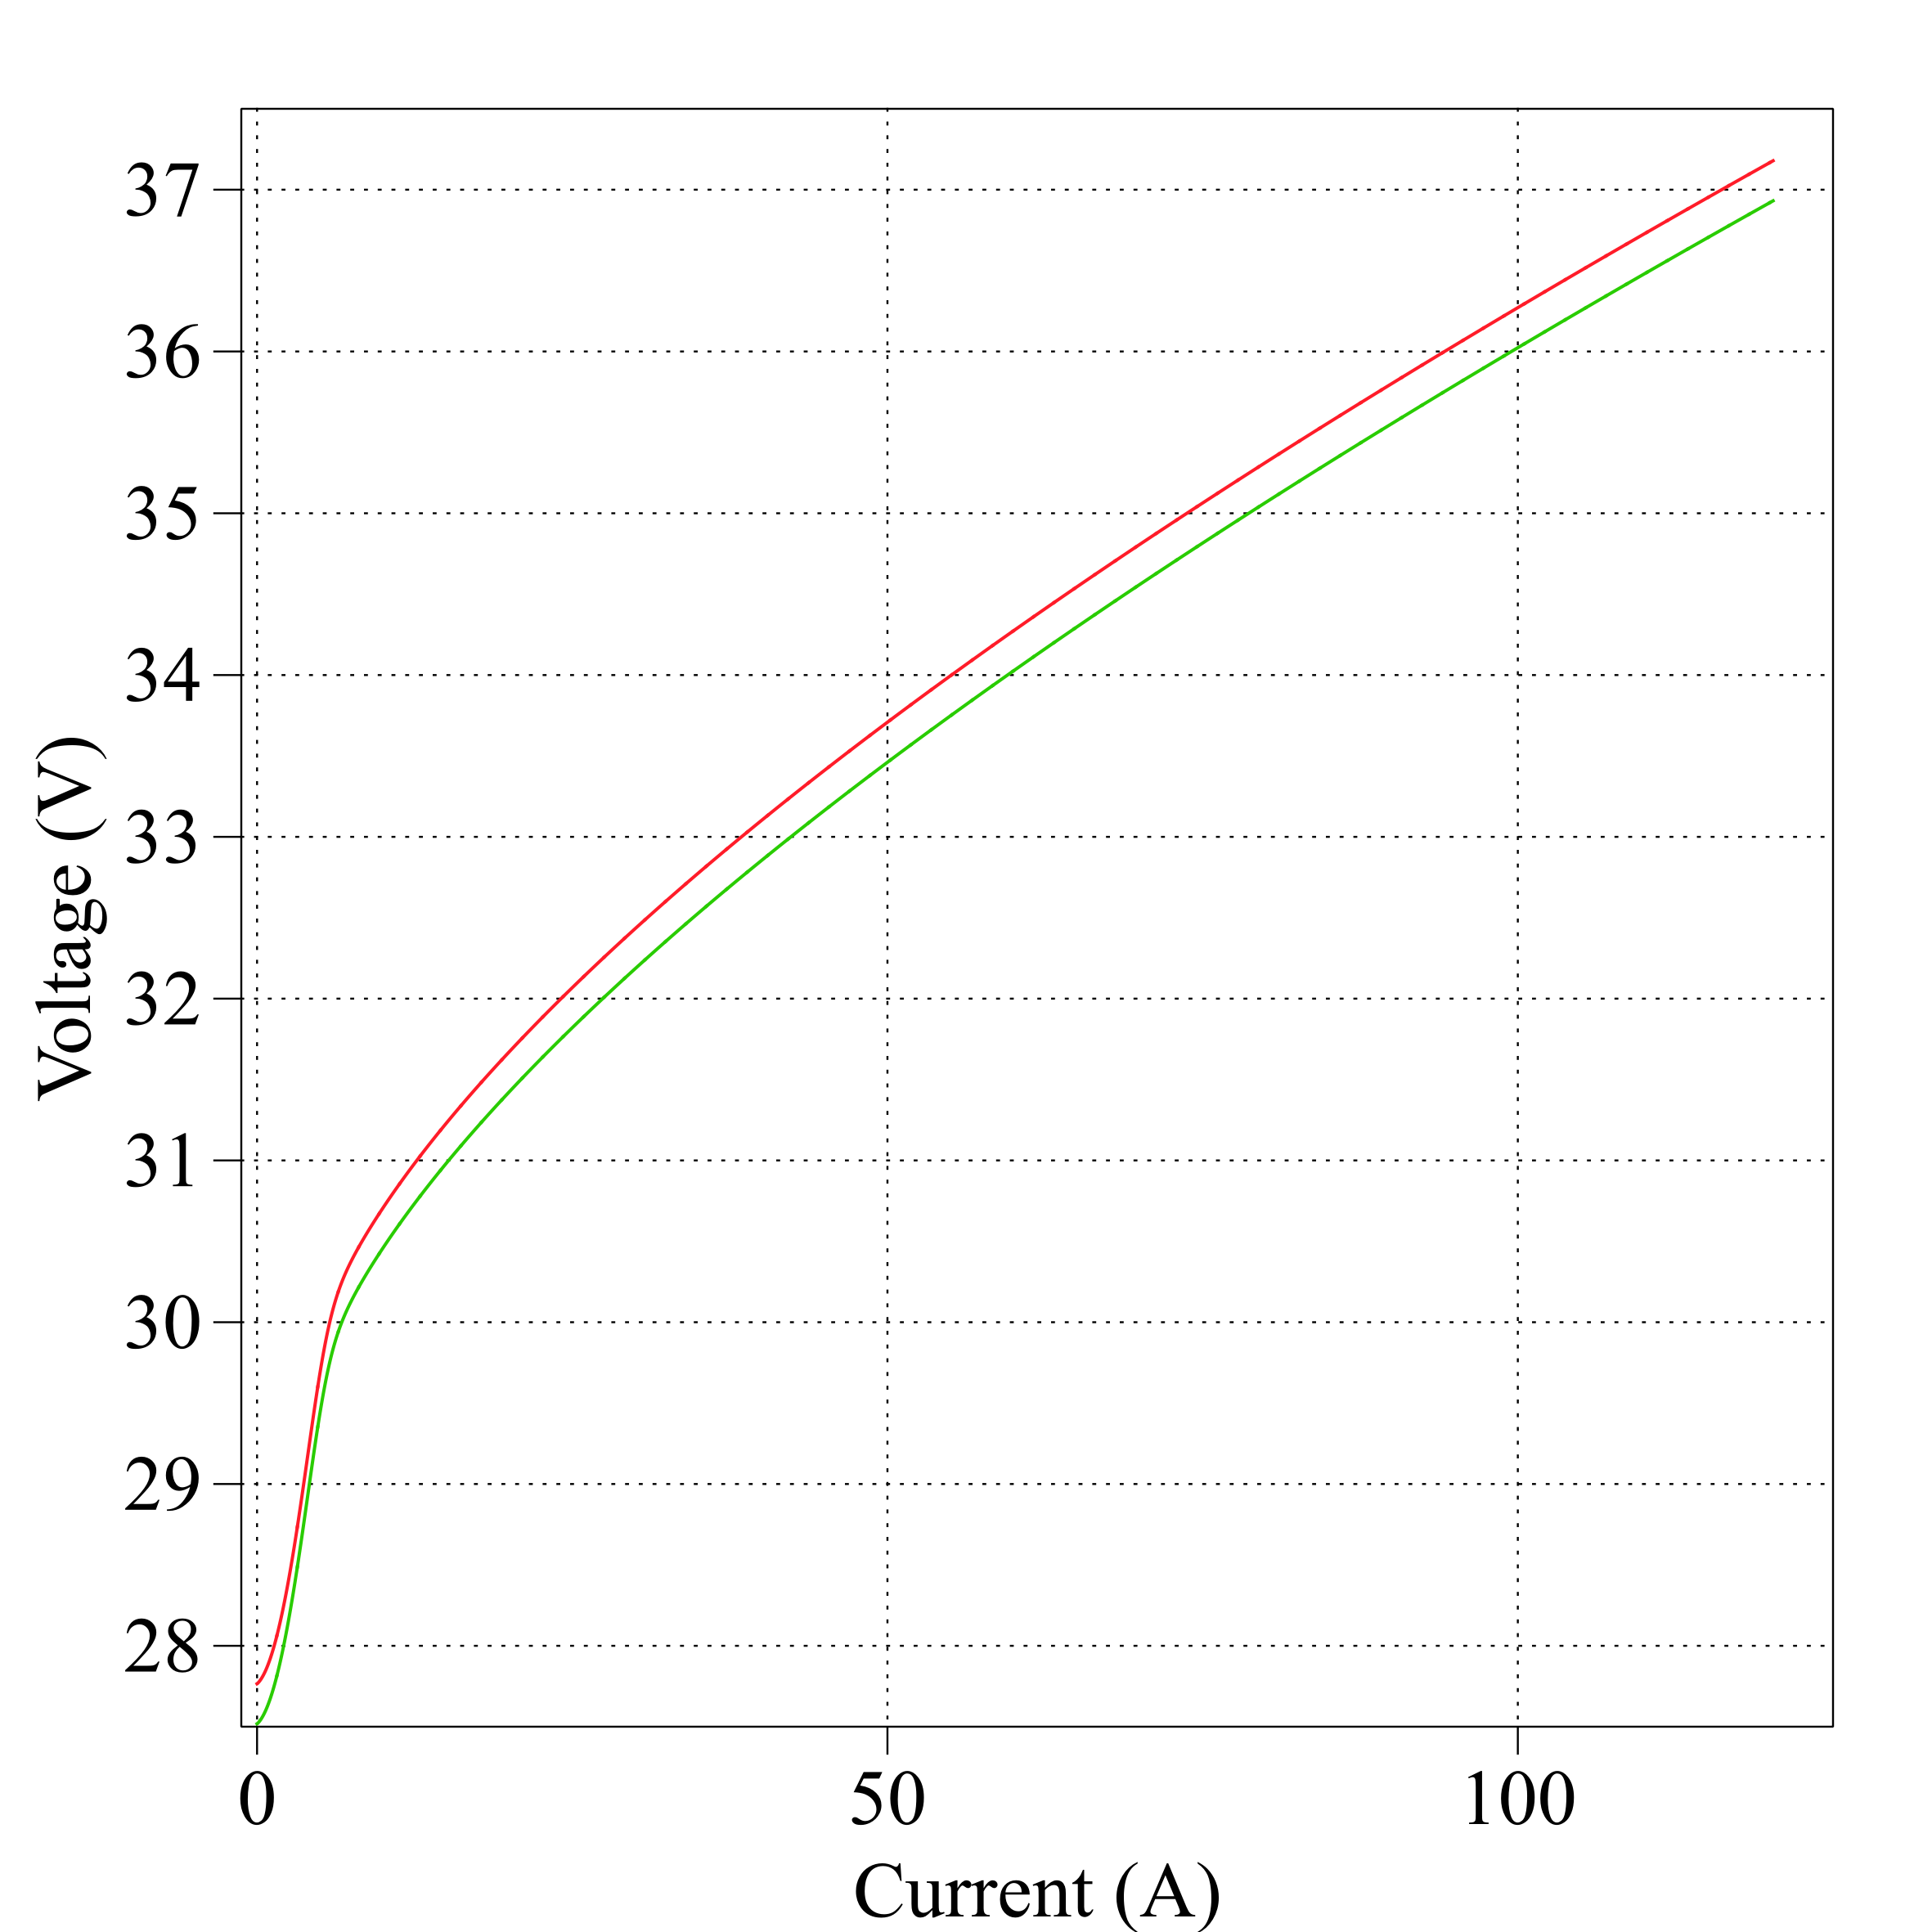
\includegraphics[scale=0.65]{scope-constant-temp.png} 
        \end{center}
      \end{column}    
    \end{columns}  
  \end{frame}    

\section{Summary}
 
  \begin{frame}{Summary}
   \begin{itemize}
    \item Brief overview of green hydrogen technology \vspace{0.3Em}
    \item Discussed on basics of electrolysis and different types 
    of electrolyzer technology currently available \vspace{0.3Em}
    \item Demonstrated an electrical equivalent circuit to portray the nonlinear and 
        dynamic behaviors of electrolyzers \vspace{0.3Em}
    \item Briefly explained various components of the electrical model \vspace{0.3Em}     
   \end{itemize}
  \end{frame}

  % \begin{frame}
  %   \begin{center}
  %     {\fontsize{30}{30}\selectfont Thank you!}
  %   \end{center}
  % \end{frame}

\end{document}